\documentclass[10pt,english]{beamer}
%\documentclass[english,handout]{beamer} % For handouts
\usetheme[progressbar=frametitle,block=fill]{metropolis} %numbering=none

%%% USEFUL PACKAGES
%\usepackage{showframe} % For debugging positioning
\usepackage{etex} % If too many packages
% Encoding and language
\usepackage[utf8]{inputenc}
\usepackage{babel}
\usepackage{amsmath, amssymb}
\usepackage{natbib}
%\usepackage{booktabs}
%\usepackage{algorithmic}
\usepackage{algorithm}
\usepackage{caption}
%\usepackage{animate} % Animations
\usepackage{bm} % Bold math
\usepackage{bbm}
%\usepackage{url}
%\usepackage{pifont}
%\usepackage{ulem} % Used for strikeouts \sout
%\usepackage{stackengine}
%\usepackage{enumitem}
%\setlist[description]{leftmargin=\parindent,labelindent=\parindent}
%\usepackage{colortbl} % Used for colored rows in tables


%%% GRAPHICS
\usepackage{graphicx}
\graphicspath{{./figs/}}


%%% COLORS
\setbeamercolor{background canvas}{bg=white}
\def\BlankFrame{
	\bgroup
	%\pdfpageheight 29.7cm
	\setbeamercolor{background canvas}{bg=}
	\begin{frame}[plain]
	\end{frame}
	%\makeatletter
	%\pdfpageheight \beamer@paperheight
	%\makeatother
	\egroup}

\usepackage{xcolor}
\definecolor{DarkGreen}{HTML}{00B200}
\definecolor{LightBlue}{HTML}{0090D9}
\definecolor{gold}{rgb}{.812,.710,.231}
% Text markup
%\setbeamercolor{alerted text}{fg=red}
\newcommand{\blue}[1]{\textcolor{blue}{#1}}
\newcommand{\red}[1]{\textcolor{red}{#1}}
\newcommand{\grey}[1]{\textcolor{gray}{#1}}
\newcommand{\orange}[1]{\textcolor{mLightBrown}{#1}}
\newcommand\myheading[1]{\textbf{#1}}
\newcommand\myemph[1]{\underline{\emph{#1}}}
\newcommand\textexample[1]{\textit{\textbf{#1}}}

%%% SPACING
\newcommand\vws[1][1]{\vspace{#1\baselineskip}} % vertical white space
%\newcommand\strt[1][1.5ex]{\rule[-.05\baselineskip]{0pt}{#1}} % strut
\newcommand\strt[2]{\rule[-#1ex]{0pt}{#2ex}} % strut
\newcommand\Hrule{\vspace{1ex} \hrule \vspace{1ex}} % Horisontal rule with some space after

%%% MISC
\newcommand\articleref[4]{\noindent\begin{minipage}[t]{0.04\textwidth}
		\vspace{0pt} 
		\pgfuseimage{beamericonarticle}
	\end{minipage}%
	\begin{minipage}[t]{0.96\textwidth}
		\vspace{0pt}
		#1. \textbf{#2.} \textit{#3}, #4.
	\end{minipage}}

%%% METROPOLIS THEME SPECIFIC
\makeatletter
\setlength{\metropolis@progressonsectionpage@linewidth}{1pt}
\makeatother
%\setbeamercolor{progress bar}{fg=red,bg=red!50}


%%% TEXTPOS
\usepackage[absolute,overlay]{textpos} % option showboxes is useful in draft mode
\setlength{\TPHorizModule}{\paperwidth}
\setlength{\TPVertModule}{\paperheight}
\textblockorigin{0pt}{10mm} % start everything at top-left, below gray 


%%% TIKZ/PGFPLOTS
\usepackage{tikz}
\usetikzlibrary{arrows,positioning,calc,shapes.geometric}
%\usetikzlibrary{arrows,calc,shapes.geometric,decorations.pathmorphing,backgrounds,positioning,fit,petri,decorations.pathreplacing}
%\usepackage{pgfplots}
%\pgfplotsset{compat = 1.3}


%%% BLOCKS AND BOXES
% Changing colors of blocks
%\setbeamercolor{block title alerted}{bg=UURed,fg=palette primary.fg}
%\setbeamercolor{block body alerted}{bg=UURed!15}
\setbeamercolor{block title alerted}{bg=mLightBrown,fg=palette primary.fg}
\setbeamercolor{block body alerted}{bg=mLightBrown!15}
%\setbeamercolor{block title example}{bg=UUGreen,fg=palette primary.fg}
%\setbeamercolor{block body example}{bg=UUGreen!10}
% \mybox is a rectangular box
\usepackage{boxedminipage}
\setlength\fboxrule{2pt}
\setlength\fboxsep{2\fboxsep}
\newcommand\mybox[3][\textwidth]{
  {\color{#2}
    \begin{boxedminipage}{#1}
      {\color{palette primary.bg} #3}
    \end{boxedminipage}}%
}   
\usepackage{tcolorbox}
\tcbset{arc=1mm,grow to left by=3mm,grow to right by=3mm,left=2mm}
%\newenvironment{redbox}{%
%	\begin{tcolorbox}[colback=UURed!15,colframe=UURed]}{%
%	\end{tcolorbox}}
%\newenvironment{greenbox}{%
%	\begin{tcolorbox}[colback=UUGreen!15,colframe=UUGreen]}{%
%	\end{tcolorbox}}
\newenvironment{redbox}{%
	\begin{tcolorbox}[colback=red!15,colframe=red]}{%
	\end{tcolorbox}}
\newenvironment{greenbox}{%
	\begin{tcolorbox}[colback=DarkGreen!15,colframe=DarkGreen]}{%
	\end{tcolorbox}}
\newenvironment{graybox}{%
	\begin{tcolorbox}[colback=mDarkTeal!5,colframe=mDarkTeal]}{%
	\end{tcolorbox}}
\newenvironment{orangebox}{%
\begin{tcolorbox}[colback=mLightBrown!15,colframe=mLightBrown]}{%
	\end{tcolorbox}}
\newenvironment{bwbox}{%
	\begin{tcolorbox}[colback=white,colframe=black]}{%
\end{tcolorbox}}
\newenvironment{bluebox}{%
	\begin{tcolorbox}[colback=LightBlue!15,colframe=LightBlue]}{%
\end{tcolorbox}}


%%%%%%%%% NEW MACROS

\newcommand\imp[1]{\alert{\textbf{#1}}}
\newcommand\bfit[1]{\textbf{\textit{#1}}}
\newcommand\good{\color{DarkGreen}{$\blacktriangle$}} % used in lists
\newcommand\bad{\color{red}{$\blacktriangledown$}} % used in lists


\RequirePackage{amsmath, amssymb}
\RequirePackage{bbm}
%\RequirePackage{newtxmath}


% Convenience macro for referring to data source
\newcommand\sourceurl[2]{\small \grey{Data from \href{#1}{#2}}}

% Abbreviations
\RequirePackage{xspace}
\newcommand\pdf{pdf\xspace}
\newcommand\ifft{iff\xspace}
\newcommand\ex{\textbf{ex)}\xspace}

% General time series notation
\newcommand\T{n}  % Length of time series
\newcommand\rtheta{{\red{\theta}}}  % Parameter (color coded)
\newcommand\rthetah{{\red{\widehat\theta}}}  % Estimate (color coded)

% Neural netowkrs
\newcommand\h{\mathbf{h}} % Hidden state variable
\newcommand\zz{\mathbf{z}} % Generic input (vector)

% For OLS/AR
\newcommand\noise{\varepsilon}  % This is the noise in AR, but should it be the same as measurement noise in SSM?
\newcommand\noisevar{\sigma^2_\noise}
\newcommand\noisevarhat{\widehat\sigma^2_\noise}
\newcommand\X{\Phi}
\newcommand\y{\mathbf{y}}
\newcommand\bphi{\bm\phi}

% State space models
\newcommand\z{\alpha}  % State vector, general SSM
\newcommand{\obsnoise}{\varepsilon}
\newcommand{\statenoise}{\eta}
\newcommand{\varobs}{\sigma^2_{\varepsilon}}
\newcommand{\varstate}{\sigma^2_{\eta}}
% For structural time series
\newcommand{\trendnoise}{\zeta}
\newcommand{\seasnoise}{\omega}
\newcommand{\vartrend}{\sigma^2_{\trendnoise}}
\newcommand{\varseas}{\sigma^2_{\seasnoise}}

%
\newcommand\FF{T}
\newcommand\GG{R}
\newcommand\HH{Z}
\newcommand{\covobs}{\sigma_\epsilon^2}
\newcommand{\covstate}{Q}
\newcommand\initmean{a_1}
\newcommand\initcov{P_1}
% Kalman filter
\newcommand{\zpart}[2]{\z_{#1}^{#2}}
\newcommand{\wgt}[2]{\omega_{#1}^{#2}}
\newcommand{\wgtsum}[1]{\Omega_{#1}}
\newcommand\zhat[2]{\hat\z_{#1|#2}}
\newcommand\Phat[2]{P_{#1|#2}}
\newcommand\zpred[1]{\zhat{#1}{#1-1}}
\newcommand\Ppred[1]{\Phat{#1}{#1-1}}
\newcommand\zfilt[1]{\zhat{#1}{#1}}
\newcommand\Pfilt[1]{\Phat{#1}{#1}}
\newcommand\ypred[1]{\hat y_{#1|#1-1}}
\newcommand\Spred[1]{F_{#1|#1-1}}
\newcommand\Spredinv[1]{\Spred{#1}^{-1}}
\newcommand\epshat[2]{\hat{\obsnoise}_{#1|#2}}
\newcommand\etahat[2]{\hat{\statenoise}_{#1|#2}}

\newcommand{\statefun}{T}
\newcommand{\obsfun}{Z}
\newcommand{\estfun}{h}

\newcommand{\qd}{q} %State density
\newcommand{\md}{g} %Measure density

\newcommand{\rmd}{\mathrm{d}}

% SMC
\newcommand{\Np}{N}           % Number of particles
\newcommand{\Mp}{M}           % Number of particles in backward simulation



%\RequirePackage{color}
%\newcommand{\flnote}[1]{{\color{red}\textbf{[#1]}}} % Used for notes in text - color red
%\newcommand\Hrule{\vspace{1ex} \hrule \vspace{1ex}} % Horisontal rule with some space after; This is moved to beamer preamble

%%%%%%%%%%%%%%%%%%%%%%%%%%%%%%%%%%%%%%%%%%%%%%%%%%%%%%%%%%%%%%%%%%%%%%%%%%%%%%%%
%                            COMMANDS IN TEXT                                  %
%%%%%%%%%%%%%%%%%%%%%%%%%%%%%%%%%%%%%%%%%%%%%%%%%%%%%%%%%%%%%%%%%%%%%%%%%%%%%%%%
\newcommand\numtext[2]{#1\textsuperscript{#2}}
\newcommand\thsnd[1]{\ensuremath{#1\thinspace000}}
\newcommand{\peqref}[1]{\eqref{#1} on page~\pageref{#1}} % Page referencing for equations: "(1) on page 1"

%%%%%%%%%%%%%%%%%%%%%%%%%%%%%%%%%%%%%%%%%%%%%%%%%%%%%%%%%%%%%%%%%%%%%%%%%%%%%%%%
%                            SPECIFIC MATH                                     %
%%%%%%%%%%%%%%%%%%%%%%%%%%%%%%%%%%%%%%%%%%%%%%%%%%%%%%%%%%%%%%%%%%%%%%%%%%%%%%%%
% Models etc.
%\newcommand{\T}{T}            % Number of samples in data record
\newcommand{\parspace}{\Theta}                                   % Parameter space
\newcommand{\parameter}{\theta}                                  % Parameter
% Spaces
\newcommand{\setX}{\ensuremath{\mathsf{X}}}                      % State-space X
\newcommand{\sigmaX}{\ensuremath{\mathcal{X}}}                   % Sigma algebra on X
\newcommand{\setY}{\ensuremath{\mathsf{Y}}}                      % State-space Y
\newcommand{\sigmaY}{\ensuremath{\mathcal{Y}}}                   % Sigma algebra on Y
\newcommand{\setZ}{\ensuremath{\mathsf{Z}}}                      % State-space Z
\newcommand{\sigmaZ}{\ensuremath{\mathcal{Z}}}                   % Sigma algebra on Z

%%%%%%%%%%%%%%%%%%%%%%%%%%%%%%%%%%%%%%%%%%%%%%%%%%%%%%%%%%%%%%%%%%%%%%%%%%%%%%%%
%                           GENERAL MATH                                       %
%%%%%%%%%%%%%%%%%%%%%%%%%%%%%%%%%%%%%%%%%%%%%%%%%%%%%%%%%%%%%%%%%%%%%%%%%%%%%%%%

% ======== Miscellaneous symbols ========
\newcommand\eqdef{:=}
\newcommand\defeq{=:}
\newcommand\const{\text{const.}}
%\newcommand\eqdef{\stackrel{\text{\scriptsize def}}{=}}

\newcommand\iid{iid}
\newcommand{\iidsim}{\stackrel{\text{\iid}}{\sim}} % iid simulation
\newcommand{\process}[1]{\{#1\}_{t\geq 1}}       % Process (time index t)
\newcommand{\range}[2]{#1, \, \dots, \, #2}      % Range = 1, ..., N
\newcommand{\crange}[2]{\{#1, \, \dots, \, #2\}} % Curly range = {1, ..., N}
\newcommand{\prange}[2]{(#1, \, \dots, \, #2)}   % Parenthesised range = (1, ..., N)
\newcommand{\bwdrange}[2]{#1 : -1 : #2}          % Range = N, ..., 1
\newcommand{\approxpropto}{\stackrel{\sim}\propto}

% Tight dots between \int and \int in a multidimensional integral
\newcommand{\tightcdots}{\hspace*{-0.38em}\cdot\hspace*{-0.3em}\cdot\hspace*{-0.3em}\cdot\hspace*{-0.38em}}

% Arrows - convergence and mappings
% \mapsto                                                     % Mappings, x \mapsto f(x)
\newcommand{\fromto}{\rightarrow}                             % Mapping from set A to set B; f: A \fromto B
\newcommand{\goesto}{\rightarrow}                             % limits used in n \goesto \infty
\newcommand{\goestosmall}{\to}                                % limits used in \lim_{n \goestosmall \infty}
\newcommand{\convP}{\stackrel{\probab}\longrightarrow}        % Convergence in probability
\newcommand{\convD}{\stackrel{\textrm{D}}\longrightarrow}     % Convergence in distribution

% ======== Standard spaces  ========
\newcommand{\naturals}{\ensuremath{\mathbb{N}}}               % Natural numbers
\newcommand{\reals}{\ensuremath{\mathbb{R}}}                  % Real numbers
\newcommand{\nonnegatives}{\reals_{\smaller +}}               % Nonnegative numbers
\newcommand{\positives}{\reals_{\smaller ++}}                 % Positive numbers
\newcommand{\nonnegativedefinites}[1]{S_{\smaller +}(#1)}     % Nonnegative #1 x #1 matrices
\newcommand{\positivedefinites}[1]{S_{++}(#1)}                % Positive #1 x #1 matrices

% ======== Matrices ========
\newcommand{\eye}[1]{I_{#1}}                     % Identity matrix
\newcommand{\+}{\mathsf{T}}                      % Transpose
\newcommand{\kronecker}{\raisebox{1pt}{\ensuremath{\otimes}}} % Kronecker product
\DeclareMathOperator*\diag{diag}
\DeclareMathOperator*\trace{tr}

% ======== Operators, calculus etc. ========
\newcommand{\Ordo}{O}                            % Big ordo
\newcommand{\supnorm}[1]{\|#1\|_\infty}          % Supremum norm
\newcommand\osc{\text{osc}}                      % Oscillator norm
\newcommand{\grad}{\nabla}                       % Gradient
\newcommand{\complementof}[1]{\ensuremath{#1^\mathsf{c}}} % Set complement
\renewcommand\vec{\text{vec}}
\DeclareMathOperator*\supp{supp}                          % Support
\DeclareMathOperator*\card{card}                          % Set cardinality
\DeclareMathOperator*\rank{rank}                          % Rank
\DeclareMathOperator*\sign{sign}                          % Signum function
\DeclareMathOperator*\argmax{arg\,max}
\DeclareMathOperator*\argmin{arg\,min}

% ======== Probability ========
\newcommand{\Prb}{\ensuremath{\mathbb{P}}}                       % Probability
\newcommand{\E}{\ensuremath{\mathbb{E}}}                         % Expectation
\newcommand{\var}{\ensuremath{\mathrm{Var}}}                     % Variance
\newcommand{\cov}{\ensuremath{\mathrm{Cov}}}                     % Covariance
\newcommand{\cor}{\ensuremath{\mathrm{Corr}}}                     % Correlation
\newcommand{\I}{\ensuremath{\mathbbm{1}}}						 % Indicator function

%\newcommand{\abscont}{\ensuremath{\ll}}          % Absolute continuity
\renewcommand\mid{\,\vert\,} % I don't really like that \mid produces rubber lengths. Sometimes, we get very large white spaces p(x    |   y), and it can produce line breaks after "p(x |" . Is the non-rubber definition here better?
\newcommand\Mid{\,\middle\vert\,} % Stretchable |, to use with \left \right - N.B. This produces a longer | in general. Does that look better than a standard \mid?


% Distributions
\newcommand{\N}{\ensuremath{\mathcal{N}}}        % Normal
\newcommand{\uni}{\ensuremath{\mathcal{U}}}      % Uniform
\newcommand\MN{\mathcal{MN}}                     % Matrix normal
\newcommand\IW{\mathcal{IW}}                     % Inverse-Wishart
\newcommand\GP{\mathcal{GP}}                     % Gaussian process
\DeclareMathOperator*\Mult{Mult}                 % Multinomial
\DeclareMathOperator*\cat{Cat}                   % Categorical
\DeclareMathOperator*\Discrete{Discrete}         % Categorical/alternative name
\DeclareMathOperator*\bin{Bin}                   % Binomial
\DeclareMathOperator*\gam{Gam}                   % Gamma
\DeclareMathOperator*\St{St}                     % Student's t
\DeclareMathOperator*\po{Po}                   % Binomial

%\usepackage{extendedalt}
%\usepackage{animate} % Animations
%\usepackage{../lindsten}
%\usepackage{movie15}
\usepackage{tikz}
\usepackage{listofitems} % for \readlist to create arrays

\title{732G12 Data Mining}
\subtitle{Föreläsning 7}
\date{}
\author{Johan Alenlöv \\ IDA, Linköping University, Sweden}
\titlegraphic{\hfill
\includegraphics[height=1.2cm]{../LiU_primary_black.pdf}}
%\institute{Joint work with\dots}


%% MY DEF %%
\newcommand{\itm}[1]{\mathrm{Item}_{#1}}
\newcommand{\pausa}{\pause}
%\renewcommand{\pausa}{}
\tikzstyle{mynode}=[thick,draw=blue,fill=blue!20,circle,minimum size=22]


\newenvironment{nscenter}
 {\parskip=0pt\par\nopagebreak\centering}
 {\par\noindent\ignorespacesafterend}

\begin{document}

\maketitle

\begin{frame}{Dagens föreläsning}

    \begin{itemize}
        \item Introduktion
        \item K-means klustring
        \item Hierarkisk klustring
    \end{itemize}
    
\end{frame}

\begin{frame}{Projektet}
    \begin{itemize}
        \item Anmäl er till grupper på Lisam.
        \item Börja kolla på uppgiften och hitta data!
    \end{itemize}
\end{frame}

\begin{frame}{Introduktion}
    \begin{itemize}
        \item Oövervakad inlärning: Lära sig data \imp{utan} responsvariabel!
        \item Flera olika algoritmer:
        \begin{itemize}
            \item \imp{Klusteranalys}
            \item Associationsanalys
            \item Sekventiella mönster
            \item Dimensionalty reduction techniques
            \item PCS, Faktormodeller
            \item Representation Learning
        \end{itemize}
    \end{itemize}
\end{frame}

\begin{frame}{Introduktion}
    \begin{greenbox}
        Måler med klusteranalys är att dela upp datamaterialet i grupper (kluster) som är intressanta och/eller användbara.
    \end{greenbox}

    Vi vet inte i förväg vilka grupper som kommer att bildas.

    Ingen responsvariabel.
\end{frame}

\begin{frame}{Klusteranalys}

    Ta 5 minuter att fundera på följande frågor:

    \begin{enumerate}
        \item Hur många kluster finns det i bilden?
        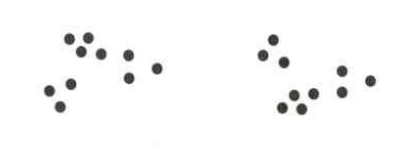
\includegraphics[width = .7\textwidth]{figs/kluster1.png}
        \item Kom på något område där klusteranalys kan vara användbart.
    \end{enumerate}
    
\end{frame}

\begin{frame}{Klusteranalys}
    
    Ett "kluster" är inte entydigt definerat.

    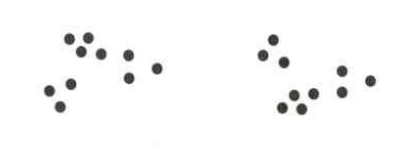
\includegraphics[width = .7\textwidth]{figs/kluster1.png}

    Tillämpningsområden:
    \begin{itemize}
        \item Biologi (toxonomi/gener)
        \item Informationssökning (Sökmotorer)
        \item Psykologi och medicin
        \item Kunddata
        \item Sociala medier/nätverk
    \end{itemize}

\end{frame}

\begin{frame}{Klassificering och klustering}

    \begin{itemize}
        \item Klassificeringsmetoder som vi jobbat med tidigare är exempel på övervakad inlärning. Ger etiketter till nya objekt, utgår från orginaldata som har etiketter.
        \item Klusteranalys är ett exempel på oövervakad inlärning - vi härleder en etikett för objekt, utgår endast från data.
    \end{itemize}
    
\end{frame}

\begin{frame}{Klustringstyper}

    \begin{description}
        \item[Partionell:] Data är indelad i ett antal oöverlappande kluster.
        \item[Hierarkisk:] Delkluster är tillåtna, kluster är representerade som ett träd.  
    \end{description}
    \vspace{1cm}
    \begin{description}
        \item[Uteslutande:] Ett objekt tillhör ett kluster.
        \item[Överlappande:] Ett objekt hör till några kluster.
        \item[Fuzzy:] Ett objekt hör till olika kluster med en specifik sannolikhet.  
    \end{description}
    \vspace{1cm}

    \begin{description}
        \item[Fullständig:] Varje objekt är tillskrivet (minst) ett kluster.
        \item[Ofullständigt:] Vissa objekt är inte tillskrivna något kluster. 
    \end{description}
    
\end{frame}

\begin{frame}{Klustertyper}
    \begin{columns}
        \begin{column}{0.5\textwidth}
            \begin{itemize}
                \item Separerade
                \item Angränsande/intilliggande
                \item Centroid- eler prototypbaserade
                \item Densitet- eller täthetsbaserade
                \item Konceptuella
            \end{itemize}
        \end{column}
        \begin{column}{0.5\textwidth}
            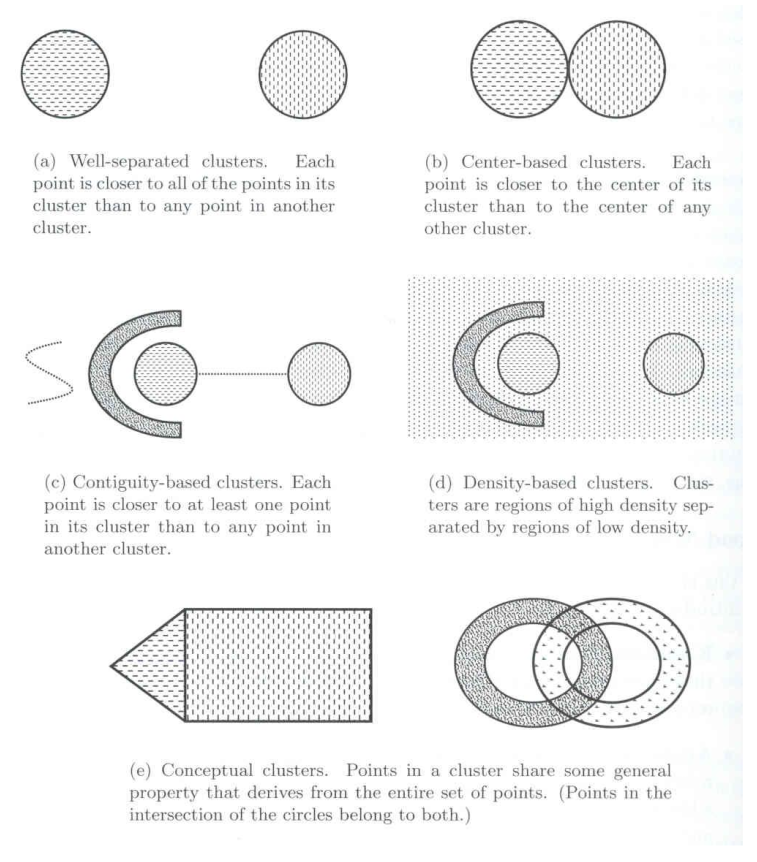
\includegraphics[width = \textwidth]{figs/Klustertyper.png}
        \end{column}
    \end{columns}
\end{frame}

\begin{frame}{K-means klustring}

    \begin{itemize}
        \item Centroid-baserad och partionell klustringsmetod.
        \begin{itemize}
            \item Centroid är en punkt som ska representera/sammanfatta alla observationer i ett kluster.
        \end{itemize}
        \item Enkel och ofta effektiv metod.
        \item $K$: hyperparameter, antalet klasser.
    \end{itemize}

    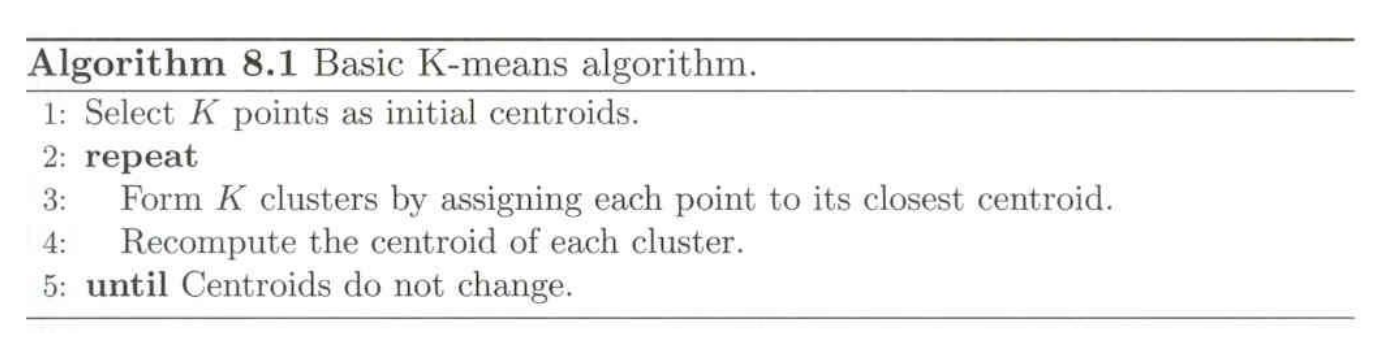
\includegraphics[width=\textwidth]{figs/basic K-means.png}
    
\end{frame}

\begin{frame}{K-means klustring}

    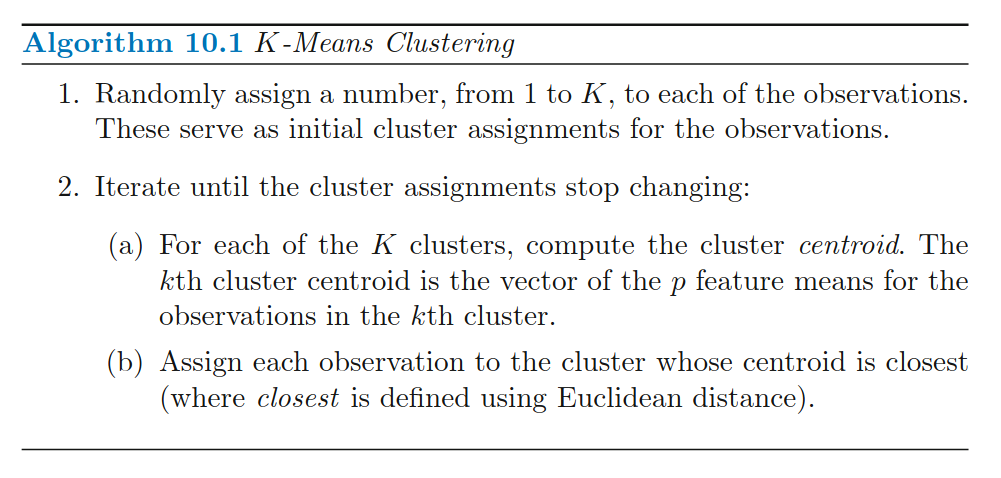
\includegraphics[width=\textwidth]{figs/K-means clustering.png}
    Från An Introduction to Statistical Learning with Applications in R av Gareth James, Daniela Witten, Trevor
Hastie, Robert Tibshirani
    
\end{frame}

\begin{frame}{K-means klustring: Exempel}
    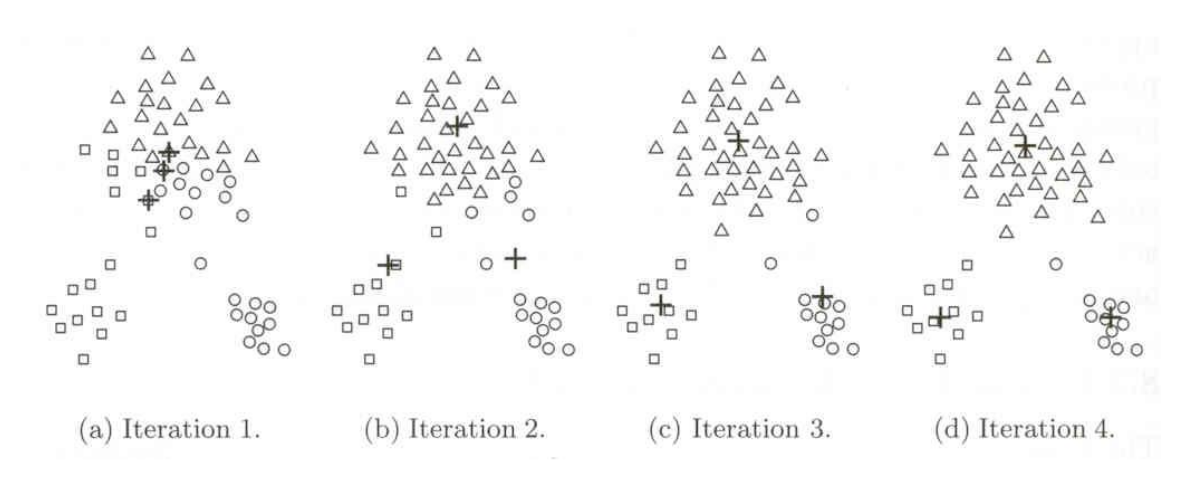
\includegraphics[width=1.1\textwidth]{figs/k-means Illustration1.png}
\end{frame}

\begin{frame}{K-means klustring: Detaljer}

    \begin{itemize}
        \item Låt $c_i$ vara centroid för kluster $i$. Låt $C_i$ vara en mängd med alla observationer i kluster $i$.
        \item Vi behöver ett avståndsmått
        \begin{itemize}
            \item Används för att mäta avståndet mellan $c_i$ och övriga observationer.
            \item Vanligast är euklidiskt avstånd,
            \begin{equation*}
                d(p,q) = \sqrt{\sum_{i=1}^{n}(q_i - p_i)^2}
            \end{equation*}
            \item Finns såklart många andra val som kan göras.
        \end{itemize}
    \end{itemize}
    
\end{frame}

\begin{frame}{K-means klustring: Detaljer}

    \begin{itemize}
        \item K-means minimerar SSE
        \item SSE i ett kluster ges av
        \begin{equation*}
            E_{c_i} = \sum_{x \in C_i} d(x, c_i)^2.
        \end{equation*}
        \item Totala SSE för alla kluster
        \begin{equation*}
            \operatorname{SSE} = \sum_{i=1}^{K} E_{c_i} = \sum_{i=1}^{K} \sum_{x \in C_i} d(x, c_i)^2
        \end{equation*}
        \item I det euklidiska rummet beräknas centroider som
        \begin{equation*}
            c_i = \frac{1}{n_i} \sum_{x \in C_i} x.
        \end{equation*}
        \item K-means algoritmen hittar ett lokalt minima.
    \end{itemize}
    
\end{frame}

\begin{frame}{K-means klustring: Exempel}

    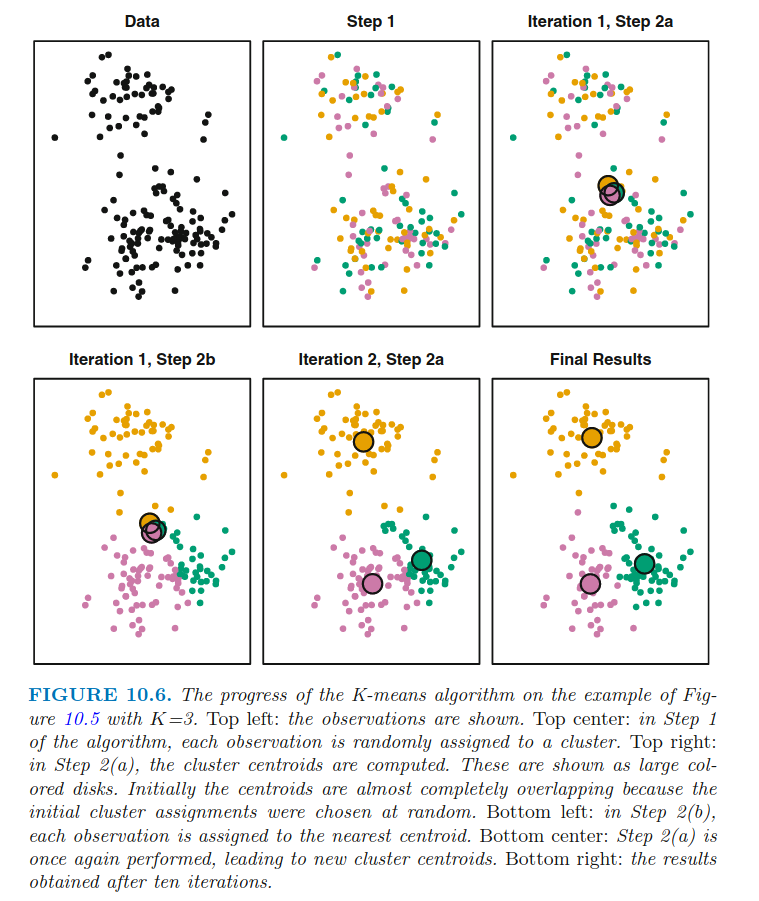
\includegraphics[height=\textheight]{figs/k-means Illustration2.png}
    
\end{frame}

\begin{frame}{K-means klustring: Startvärden}

    Vi måste välja våra initiala gissningar för centroider. Detta val påverkar starkt utgången av algoritmen.

    Dåliga startvärden kan ge dåliga resultat.
    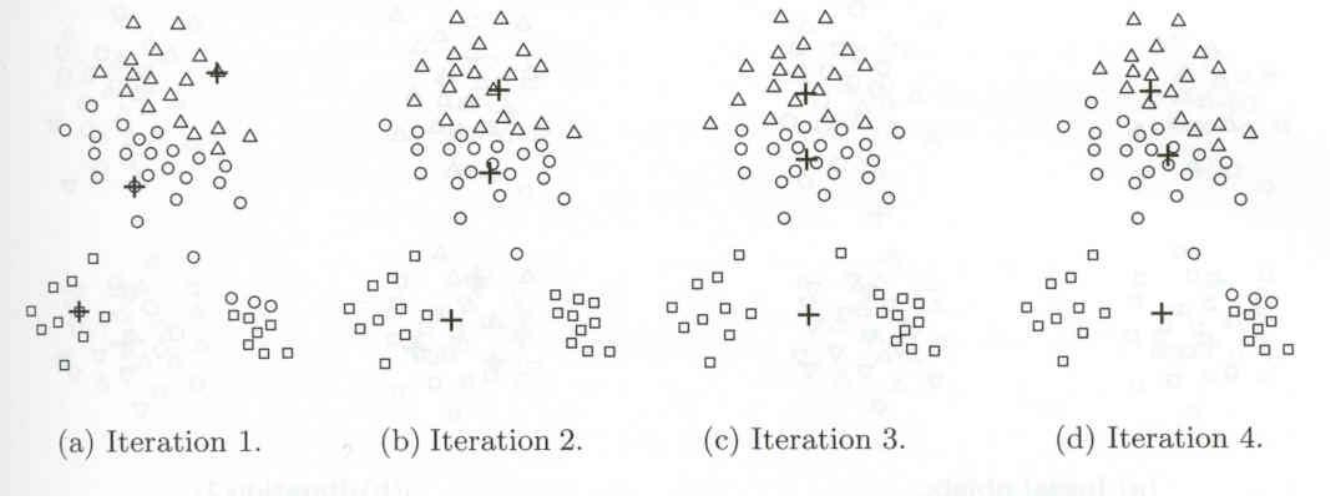
\includegraphics[width = \textwidth]{figs/dåliga start värden.png}

    Vanlig metod är att köra algoritmen många gångenr med olika (slumpade) startvärden.
    
\end{frame}

\begin{frame}{Halverande K-means}

    \begin{itemize}
        \item Algoritm som motverkar problemet med startvärden.
        \item Dela upp datamängden i två kluster, välj ett och dela upp det i två osv.
        \begin{itemize}
            \item Valet av kluster kan göras med avseende på flest observation, störst SSE eller annat kriterie.
        \end{itemize}
        \item Uppdelningen kan liknas vid ett binärt träd.
    \end{itemize}
    
\end{frame}

\begin{frame}{Halverande K-means}

    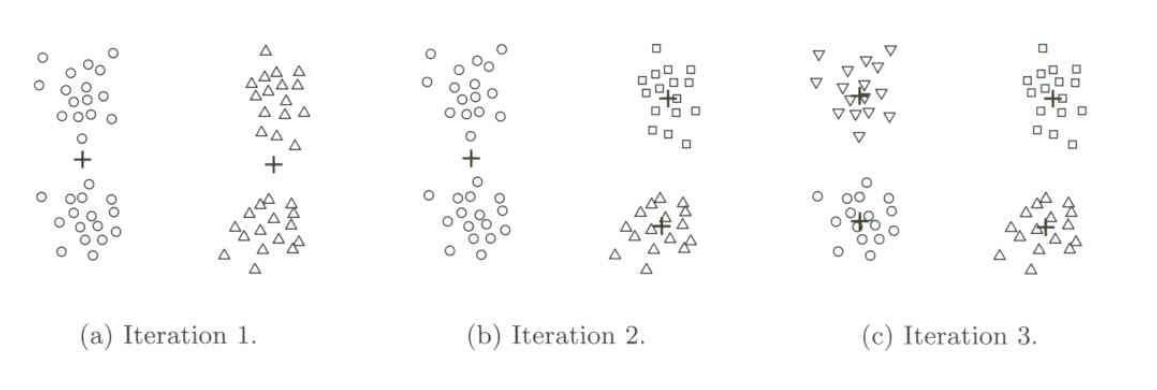
\includegraphics[width=\textwidth]{figs/Halverande K-means_exempel.png}
    
\end{frame}

\begin{frame}{Halverande K-means}

    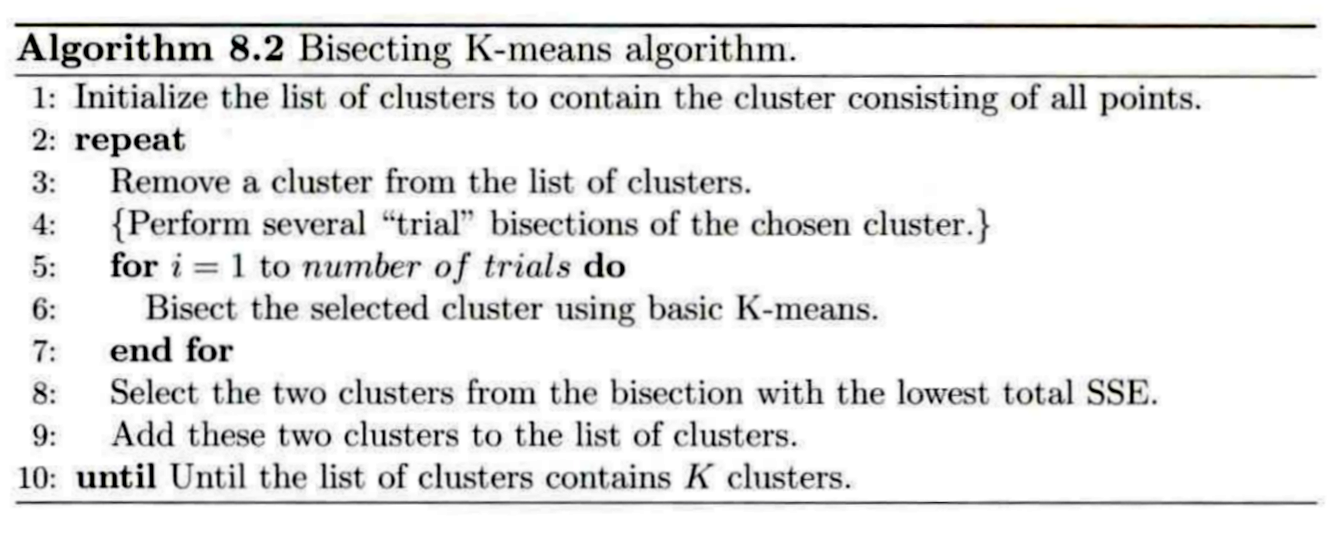
\includegraphics[width = \textwidth]{figs/Halverande K-means algoritm.png}
    
\end{frame}

\begin{frame}{K-means++}


    Algoritm för att hitta startvärden till K-means.

    \begin{enumerate}
        \item Välj en centroid uniformt slumpmässigt från observationerna.
        \item För varje datapunkt $x$ beräkna avstånder $d(x,c_i)$ mellan $x$ och den närmaste centroiden (som redan valts).
        \item Välj en datapunkt som centroid genom att:
        \begin{itemize}
            \item Slump en punkt med hjälp av viktade sannolikheter, där vikterna är proportionella mot $d(x,c_i)^2$.
        \end{itemize}
        \item Upprepa 2 och 3 tills $K$ centroider valts ut.
        \item Kör vanlig K-means med dessa startcentroider.
    \end{enumerate}
    
\end{frame}

\begin{frame}{K-means++}

    \begin{itemize}
        \item Generellt: K-means++ förbättrar SSE mycket över slumpade startvärden.
        \item Tar extra tid att bestämma startvärden, men K-means konvergerar mycket snabbare än med slumpade startvärden.
        \item Vanligt att K-means++ är dubbelt så snabb som K-means med slumpade startvärden.
    \end{itemize}
    
\end{frame}

\begin{frame}{K-means klustring: Kommentarer}

    \begin{itemize}
        \item Enkel och ganska effektiv.
        \item Känslig mot startvärden.
        \begin{itemize}
            \item Kör många gånger med olika startvärden.
            \item Halverande K-means.
            \item K-means++
        \end{itemize}
        \item Skapar klotformade kluster och är linjärt separerade.
        \begin{itemize}
            \item Andra former fungerar sämre.
        \end{itemize}
        \item Ger en centroid för varje kluster. Kan användas för att beskriva klustret.
        \item Har svårt att identifiera kluster av olika storlekar eller med olika tätheter.
        \item Känslig mot extremvärden.
    \end{itemize}
    
\end{frame}

\begin{frame}{K-mean klustring: Utökningar}

    \begin{itemize}
        \item Kernel K-means: Kan forma kluster av olika former med icke-linjära separationsgränser.
        \item Gaussian mixture models/klustring:
        \begin{itemize}
            \item Varje kluster beskrivs med en multivariat normalfördelning.
            \item Skattas med expectation-maximization (EM) algoritmen.
        \end{itemize}
        \item K-medoids/Partitioning Around Medoids. Använder medioder som center (en punkt i datasetet).
        \item K-medians klustring: använder medianer istället.
    \end{itemize}
    
\end{frame}

\begin{frame}{Hierarkisk klustring}

\begin{itemize}
    \item Två typer:
    \begin{itemize}
        \item Agglomerativ, bygger underifrån.
        \item Diversiv, bygger uppifrån.
    \end{itemize}
    \item Skapar en hierarki med kluster.
    \begin{itemize}
        \item Subkluster som har subkluster som har subkluster....
    \end{itemize}
\end{itemize}    
    
\end{frame}


\begin{frame}{Agglomerativ hierarkisk klustring}

    \begin{itemize}
        \item Börja med att ge varje observation sitt egna kluster. Slå ihop närliggande kluster till ett större kluster. Upprepa detta tills alla observationer är i ett kluster.
        \item Proocessen visualiseras i ett s.k. dendogram.
        \begin{itemize}
            \item Vågrät axel innehåller observationsnummer (ordningen är odtycklig)
            \item Lodrät axel mäter avstånd mellan kluster.
            \item Förgreningen mäter vilka kluster och vid vilket avstånd dessa lås ihop.
        \end{itemize}
    \end{itemize}

    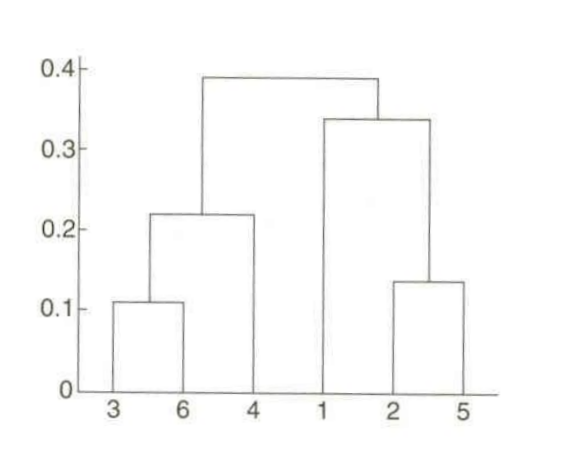
\includegraphics[width = 0.5 \textwidth]{figs/dendogram1.png}
    
\end{frame}

\begin{frame}{Agglomerativ hierarkisk klustring}

    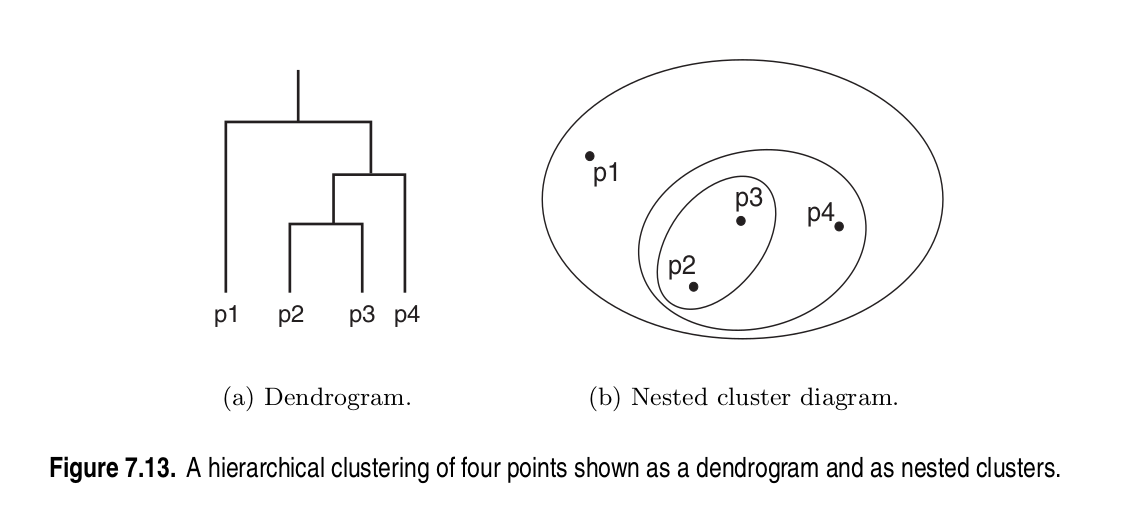
\includegraphics[width = \textwidth]{figs/dendogram2.png}
    
\end{frame}

\begin{frame}{Dendogram}

    \begin{itemize}
        \item Dendogrammet visar \imp{alla} ihopslagningar.
        \item Vi måste manuellt ange när vi anser att ihopslagningarna ska sluta: Hur många kluster?
        \begin{itemize}
            \item Subjektivt
            \item När avståndet mellan ihopslagningar är "stort nog".
        \end{itemize}
    \end{itemize}
    
\end{frame}

\begin{frame}{Dendogram}

    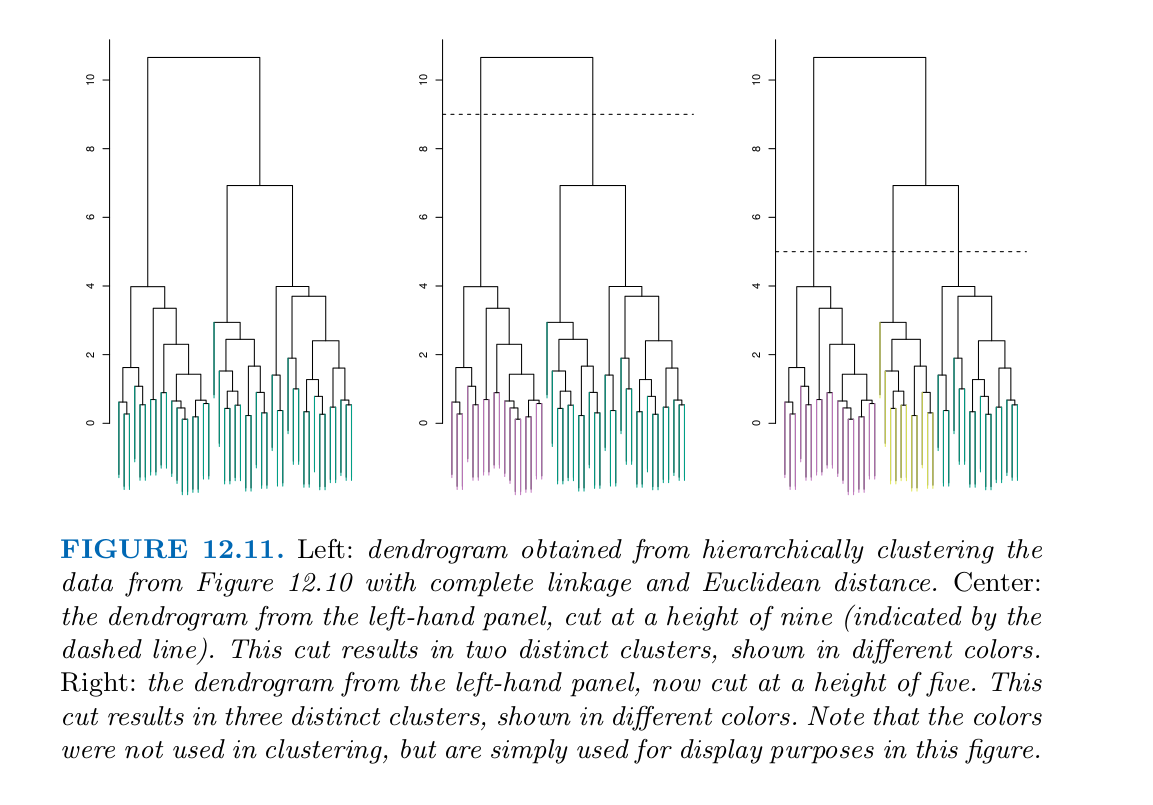
\includegraphics[width=\textwidth]{figs/dendogram3.png}
    
\end{frame}

\begin{frame}{Agglomerativ hierarkisk klustring: Algoritm}

    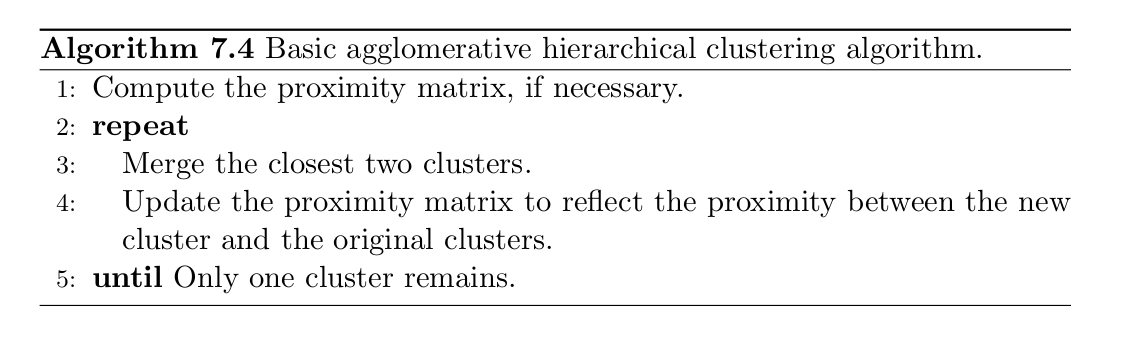
\includegraphics[width = \textwidth]{figs/hclut_alg.png}

    Proximity matrix är en matris som innehåller närheten mellan kluster. Kan använda en distansmatris också.

\end{frame}

\begin{frame}{Beräkning av avstånd mellan två kluster}

    Då kluster ofta innehåller flera observationer behövs en metod för att definera hur avstånd beräknas, även kallad \imp{länkningsmetod}.

    Låt $C_i$ och $C_j$ vara två kluster.
    \begin{itemize}
        \item MIN eller Single (enkel länkning):
        \begin{equation*}
            \operatorname{prox}(C_i, C_j) = \min_{x \in C_i, y \in C_j} \operatorname{dist}(x, y).
        \end{equation*}
        \item MAX eller Complete (fullständig länkning):
        \begin{equation*}
            \operatorname{prox}(C_i, C_j) = \max_{x \in C_i, y \in C_j} \operatorname{dist}(x, y).
        \end{equation*}
    \end{itemize}
    
\end{frame}

\begin{frame}{Beräkning av avständ mellan två kluster}

    \begin{itemize}
        \item Group average (genomsnitts länkning):
        \begin{equation*}
            \operatorname{prox}(C_i, C_j) = \frac{1}{n_i \cdot n_j} \sum_{x \in C_i, y \in C_j} \operatorname{dist}(x,y),
        \end{equation*}
        där $n_i$ och $n_j$ är antalet observationer i kluster $i$ och $j$.
        \item Wards/Centroid metod: Närheten defineras som hur mycket kvadrerade fel ökar när två kluster slås ihop.
        
        Samma kostnadsfunktion som i K-means.
    \end{itemize}
    
\end{frame}

\begin{frame}{Beräkning av avstånd mellan två kluster}

    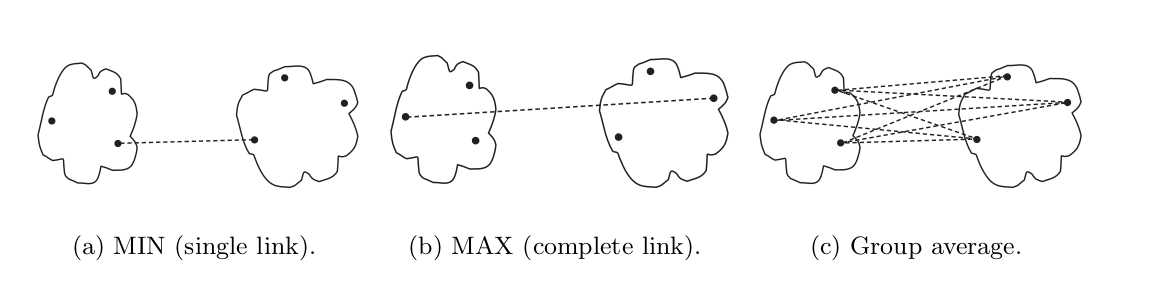
\includegraphics[width = \textwidth]{figs/linking_pic.png}
    
\end{frame}

\begin{frame}{Egenskaper}

    \begin{itemize}
        \item Ingen global funktion att optimera.
        \item Group average- och olika centroid metoder kan ta hänsyn till olika klusterstorlekar när ett par kluster förenas.
        \item Ihopslagningar är slutgiltiga och går inte att ta isär senare.
        \item Närhetsmåttet kan påverka resultatet.
        \begin{itemize}
            \item Extremvärden.
            \item Brus.
        \end{itemize}
        \item Passar bra för data som har en hierarkisk struktur.
    \end{itemize}
    
\end{frame}

\begin{frame}{Exempel}
    
    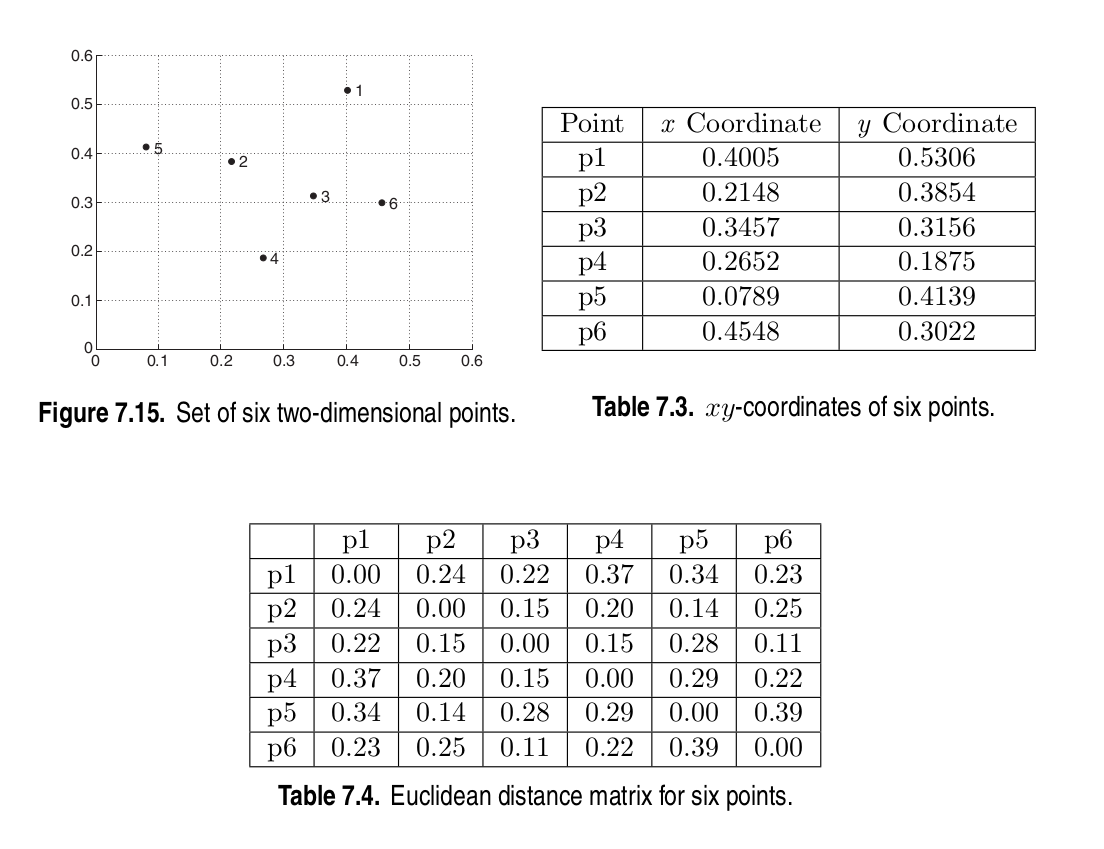
\includegraphics[width=\textwidth]{figs/ex_data.png}

\end{frame}

\begin{frame}{Exempel}

    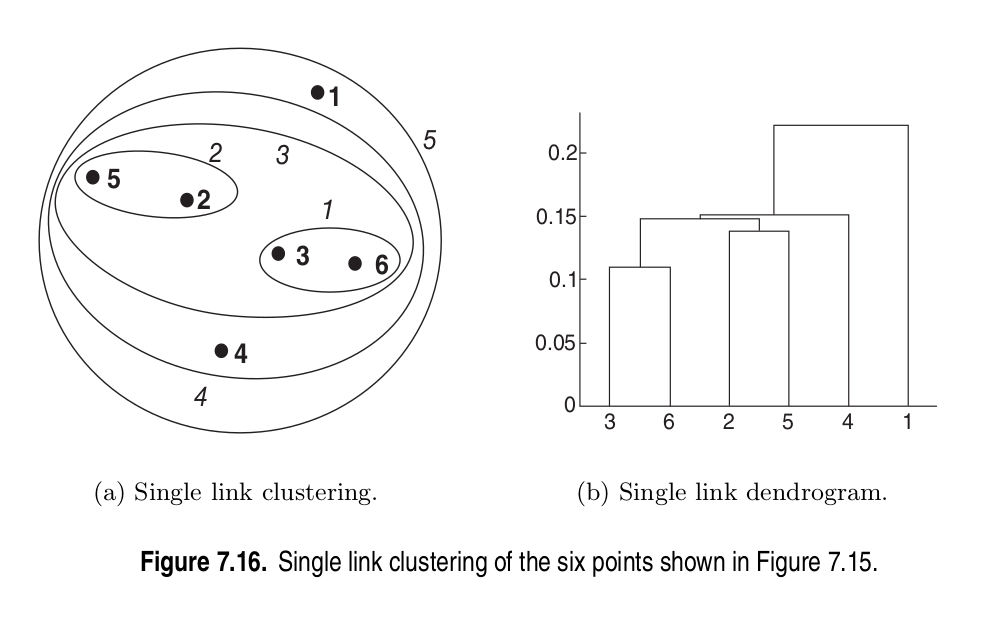
\includegraphics[width=.495\textwidth]{figs/Single link clustering.png} 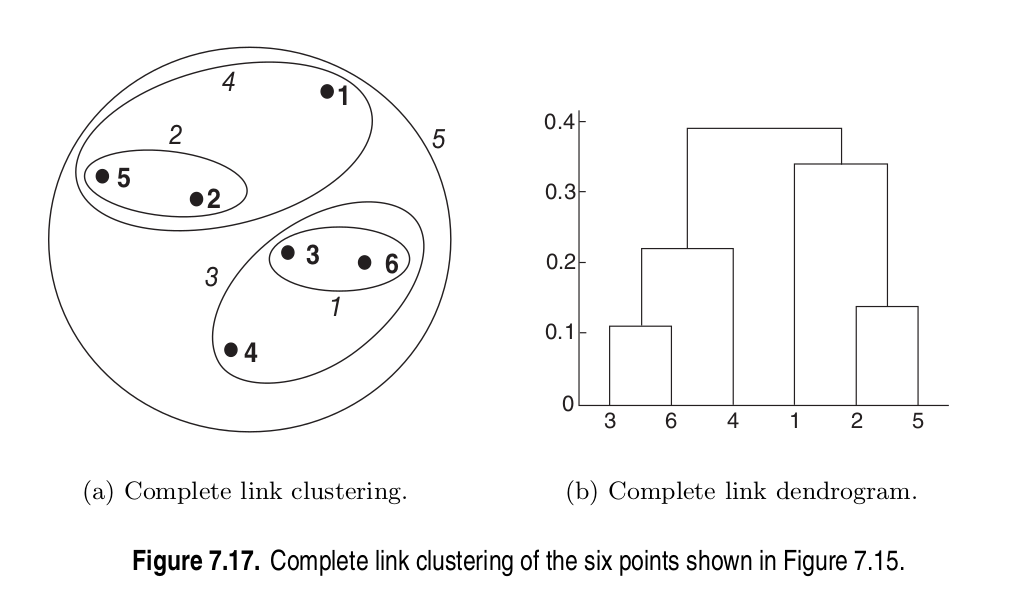
\includegraphics[width=.495\textwidth]{figs/Complete link clustering.png}
    
\end{frame}

\begin{frame}{Exempel}

    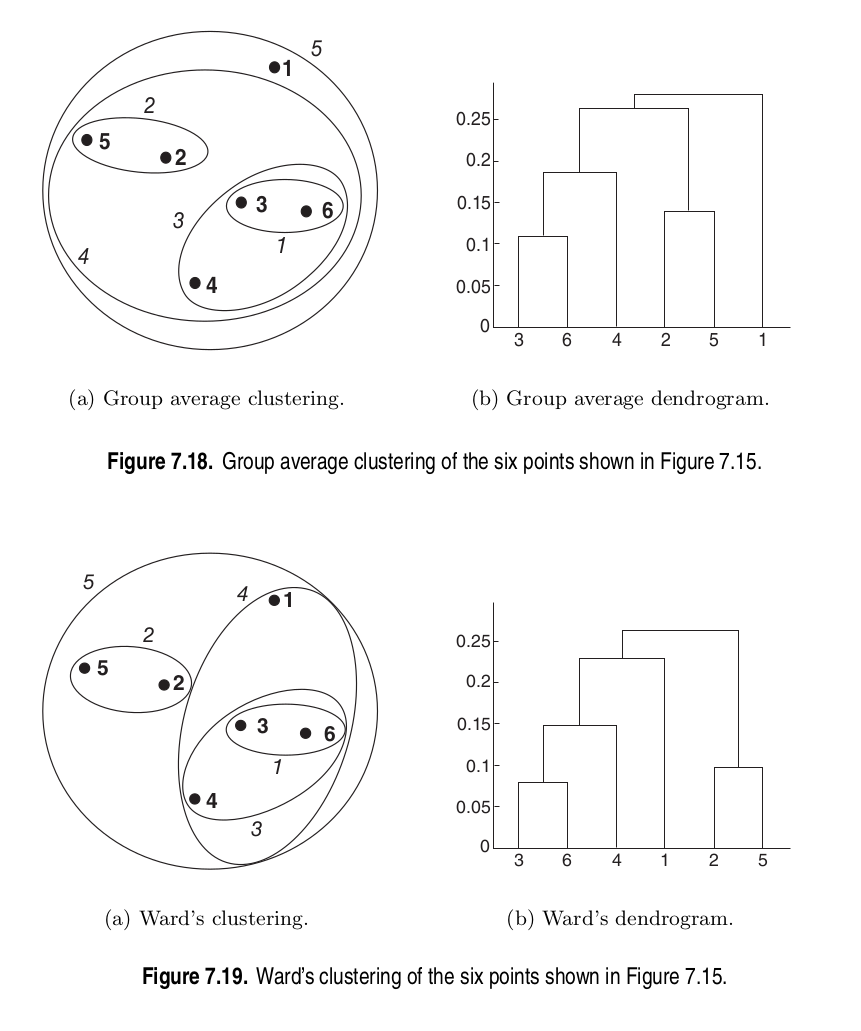
\includegraphics[height=\textheight]{figs/grouP_ward_clustering.png}
    
\end{frame}

\end{document}